%-------------------------
% Resume in Latex
% Author : Arkadeep Das, Manas Daruka, Ayush Sharma, Abhinav Gupta
% License : MIT
%------------------------

%---- Required Packages and Functions ----

\documentclass[a4paper,11pt]{article}
\usepackage{latexsym}
\usepackage{xcolor}
\usepackage{float}
\usepackage{ragged2e}
\usepackage[empty]{fullpage}
\usepackage{wrapfig}
\usepackage{lipsum}
\usepackage{tabularx}
\usepackage{titlesec}
\usepackage{geometry}
\usepackage{marvosym}
\usepackage{verbatim}
\usepackage{enumitem}
\usepackage[hidelinks]{hyperref}
\usepackage{fancyhdr}
\usepackage{multicol}
\usepackage{graphicx}
\usepackage{cfr-lm}
\usepackage[T1]{fontenc}
\setlength{\multicolsep}{0pt} 
\pagestyle{fancy}
\fancyhf{} % clear all header and footer fields
\fancyfoot{}
\renewcommand{\headrulewidth}{0pt}
\renewcommand{\footrulewidth}{0pt}
\geometry{left=1.4cm, top=0.8cm, right=1.2cm, bottom=1cm}
% Adjust margins
%\addtolength{\oddsidemargin}{-0.5in}
%\addtolength{\evensidemargin}{-0.5in}
%\addtolength{\textwidth}{1in}
\usepackage[most]{tcolorbox}
\tcbset{
	frame code={}
	center title,
	left=0pt,
	right=0pt,
	top=0pt,
	bottom=0pt,
	colback=gray!20,
	colframe=white,
	width=\dimexpr\textwidth\relax,
	enlarge left by=-2mm,
	boxsep=4pt,
	arc=0pt,outer arc=0pt,
}

\urlstyle{same}

\raggedright
\setlength{\tabcolsep}{0in}

% Sections formatting
\titleformat{\section}{
  \vspace{-4pt}\scshape\raggedright\large
}{}{0em}{}[\color{black}\titlerule \vspace{-7pt}]

%-------------------------
% Custom commands
\newcommand{\resumeItem}[2]{
  \item{
    \textbf{#1}{:\hspace{0.5mm}#2 \vspace{-0.5mm}}
  }
}

\newcommand{\resumePOR}[3]{
\vspace{0.5mm}\item
    \begin{tabular*}{0.97\textwidth}[t]{l@{\extracolsep{\fill}}r}
        \textbf{#1},\hspace{0.3mm}#2 & \textit{\small{#3}} 
    \end{tabular*}
    \vspace{-2mm}
}

\newcommand{\resumeSubheading}[4]{
\vspace{0.5mm}\item
    \begin{tabular*}{0.98\textwidth}[t]{l@{\extracolsep{\fill}}r}
        \textbf{#1} & \textit{\footnotesize{#4}} \\
        \textit{\footnotesize{#3}} &  \footnotesize{#2}\\
    \end{tabular*}
    \vspace{-2.4mm}
}

\newcommand{\resumeProject}[4]{
\vspace{0.5mm}\item
    \begin{tabular*}{0.98\textwidth}[t]{l@{\extracolsep{\fill}}r}
        \textbf{#1} & \textit{\footnotesize{#3}} \\
        \footnotesize{\textit{#2}} & \footnotesize{#4}
    \end{tabular*}
    \vspace{-2.4mm}
}

\newcommand{\resumeSubItem}[2]{\resumeItem{#1}{#2}\vspace{-4pt}}

% \renewcommand{\labelitemii}{$\circ$}
\renewcommand{\labelitemi}{$\vcenter{\hbox{\tiny$\bullet$}}$}

\newcommand{\resumeSubHeadingListStart}{\begin{itemize}[leftmargin=*,labelsep=0mm]}
\newcommand{\resumeHeadingSkillStart}{\begin{itemize}[leftmargin=*,itemsep=1.7mm, rightmargin=2ex]}
\newcommand{\resumeItemListStart}{\begin{justify}\begin{itemize}[leftmargin=3ex, rightmargin=2ex, noitemsep,labelsep=1.2mm,itemsep=0mm]\small}

\newcommand{\resumeSubHeadingListEnd}{\end{itemize}\vspace{2mm}}
\newcommand{\resumeHeadingSkillEnd}{\end{itemize}\vspace{-2mm}}
\newcommand{\resumeItemListEnd}{\end{itemize}\end{justify}\vspace{-2mm}}
\newcommand{\cvsection}[1]{%
\vspace{2mm}
\begin{tcolorbox}
    \textbf{\large #1}
\end{tcolorbox}
    \vspace{-4mm}
}

\newcolumntype{L}{>{\raggedright\arraybackslash}X}%
\newcolumntype{R}{>{\raggedleft\arraybackslash}X}%
\newcolumntype{C}{>{\centering\arraybackslash}X}%
%---- End of Packages and Functions ------

%-------------------------------------------
%%%%%%  CV STARTS HERE  %%%%%%%%%%%
%%%%%% DEFINE ELEMENTS HERE %%%%%%%
\newcommand{\name}{Huan Nguyen-Duy} % Your Name
\newcommand{\course}{BE - Computer Engineering} % Your Course
\newcommand{\phone}{86607 8421} % Your Phone Number
\newcommand{\email}{huan2931@gmail.com} %Email 1
\newcommand{\github}{Winxkin} %Github
\newcommand{\facebook}{https://www.facebook.com/xkin.win/} %Website
\newcommand{\linkedin}{huan-nguyen-duy-a7693023b} %linkedin




\begin{document}
\fontfamily{cmr}\selectfont
%----------HEADING-----------------
\parbox{2.35cm}{%

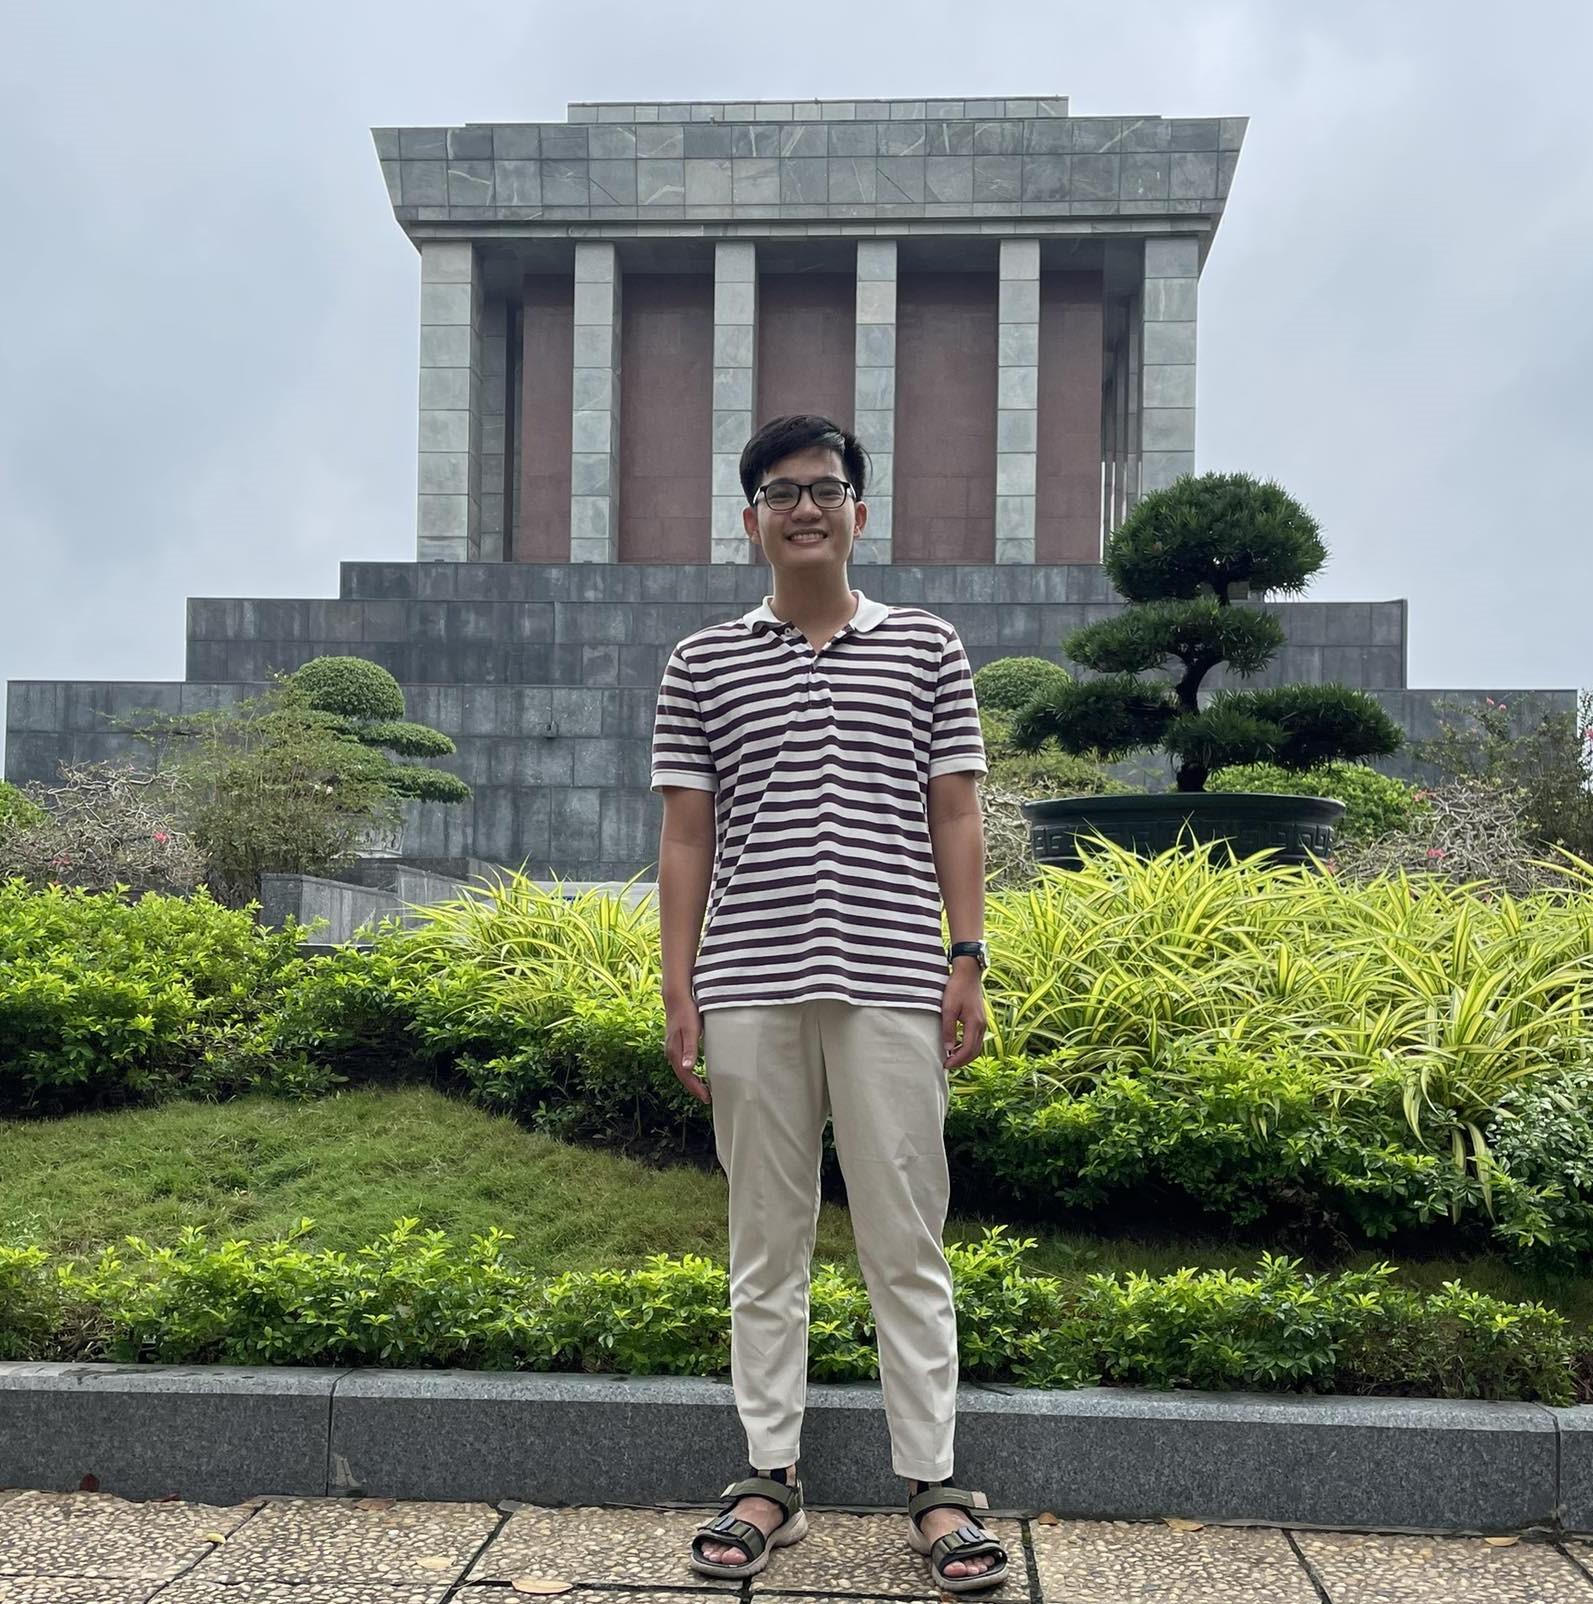
\includegraphics[width=2cm,clip]{logo.jpg}

}\parbox{\dimexpr\linewidth-2.8cm\relax}{
\begin{tabularx}{\linewidth}{L r}
  \textbf{\LARGE \name} & +84-\phone\\
%   {Roll No.:\roll} & \href{mailto:\emaila}{\emaila} \\
  \course &  \href{mailto:\email}{\email}\\
  {Engineer in Automotive industry} &  \href{https://github.com/\github}{Github} $|$ \href{\facebook}{facebook} $|$ \href{https://www.linkedin.com/in/}{linkedin}\\
  {Ho Chi Minh City University of Technology and Education, VietNam} %& \href{\Linkedln}{linkedin}
\end{tabularx}
}



%-----------EDUCATION-----------------
% \section{Education}
%   \resumeSubHeadingListStart
%     \resumeSubheading
%       {Indian Institute of Technology Guwahati}{Guwahati, India}
%       {Bachelor of Technology in Mathematics and Computing ;  GPA: 8.10}{July. 2015 -- July. 2019 (Expected)}
%     \resumeSubheading
%       {Burdwan Model School}{Burdwan, W.B}
%       {Central Board of Secondary Education (Class XII);  Percentage: 96.60}{March. 2015}
%   \resumeSubHeadingListEnd\vspace{-3mm}
\section{Education}
\setlength{\tabcolsep}{5pt} % Default value: 6pt
% \renewcommand{\arraystretch}{1.1} % Default value: 1
\small{\begin{tabularx}
{\dimexpr\textwidth-3mm\relax}{|c|C|c|c|c|}
  \hline
  \textbf{Degree/Certificate } & \textbf{Institute/Board} & \textbf{GPA} & \textbf{Year} & \textbf{Reference No}\\
  \hline
  SPK.BE. Computer Engineering & Ho Chi Minh City University of Technology and Education & 3.22 & 2023 & 2427FD23\\
  \hline
\end{tabularx}}
\vspace{-2mm}

% %-----------EXPERIENCE-----------------
\section{Experience}
  \resumeSubHeadingListStart

    \resumeSubheading
      {Ban Vien Corporation}{Ban Vien Tower, 54-56-58 Street 2, Van Phuc Residences,Thu Duc district, HCM}
      {Intern}{June 2022 - Aug 2022}
      \resumeItemListStart
    \item {Project vending machine}\hfill 
    \\ {**Programming: C,C++}
    \\ {[1] Supporting application programing interface of RFID module for STM32F1 chip.}
    \\ {[2] Supporting application programing interface of UART which is connected STM32F1 by QT framework.}
    % \item {More work done } .....
    \resumeItemListEnd
    \resumeSubheading
    {Ban Vien Corporation}{Ban Vien Tower, 54-56-58 Street 2, Van Phuc Residences,Thu Duc district, HCM}
    {Part-time Embedded Engineer}{Aug 2022 - Apr 2023}
    \resumeItemListStart
  \item {Training SOC project}\hfill
  \\ {**Programming: C, C++}
  \\ {[1] Builder tools: Makefile, poky package (Yocto project)}
  \\ {[2] learning embedded Linux that include Linux kernel, Yocto project, Linux application.}
  \\ {[3] Building custom image for Raspberry Pi 3 board.}
  \\ {[4] Expanding GPIO application with PCF8574 module by using device driver.}
  \item {Advanced Driver Assistance Systems hackathon project}\hfill
  \\ {**Programming: C++}
  \\ {[1] Integrating peripheral components into Jetson Nano by using device driver.}
  \\ {[2] Integrating module CAN mcp2510 into Jetson nano by using device driver.}
  \\ {[3] Integrating module Raspberry camera (imx219) into Jetson nano by using device driver.}
  \\ {[4] Responsibility for design role to develop CAN service, this was combine between CAN interface and DBUS service, which were supported by Linux kernel.}
  % \item {More work done } .....
  \resumeItemListEnd
    \resumeSubheading
    {Ban Vien Corporation}{Ban Vien Tower, 54-56-58 Street 2, Van Phuc Residences,Thu Duc district, HCM}
    {Embedded Engineer}{May 2023 - Present}
    \resumeItemListStart
  \item {Model base design | QEMU development project}\hfill
  \\ {***Customer: Renesas Design Vietnam Co., Ltd., Ho Chi Minh City.}
  \\ {**Bief project: QEMU development project aims the emulation for RCAR chip (development by Renesas Design Vietnam), it creates the emulation fastest platform to reduce the cost and time consumption of the development process.
        QEMU project was developed by C/Cpp programing and several opensource libraries to emulate RCAR chip series, we implemented all modules in SOC chip (RCAR series) base on hardware specifications which were provided by IC design teams.
        The ouputs of QEMU project were RCAR chip platform software series that had operations similar to real RCAR chip series (developed by IC design teams). These ouputs can called Virtual-Platform.}
  \\ {**Fundamental knowledges: modeling techniques, C/Cpp programing, Makefile.}
  \\ {[1] Model RS-CANFD : Investigating hardware specification of RS-CANFD model, preparing environment and Integrating the design of this model to virtual platform. After that, planning to create test cases to verify all operations.}
  \item {Model base design | RCAR development project}\hfill
  \\ {***Customer: Renesas Design Vietnam Co., Ltd., Ho Chi Minh City.}
  \\ {**Bief project: RCAR development project aims the simulation for RCAR chip (development by Renesas Design Vietnam), it uses mainly systemC framework to simulate accurate operations of RCAR chip base on hardware specifications which were provided by IC design teams.
        RCAR project objective provide for customer the virtual platform of SOC chip with high accurate.}
  \\ {**Fundamental knowledges: modeling techniques, systemC framework, C/Cpp programing, Makefile.}
  \\ {[1] VSP2 model (Video Signal Processor) : Investigating hardware specification provided by IC design teams and updating some registers which were changed compare with last specification version.}
  \\ {[2] SHIP-M-AES submodel (Security Advanced Encryption Standard): Investigating hardware specification provided by IC design teams, Responsibility for design dummys, preparing environment to verify AES moduel. Creating test cases to verify full opeartion of AES submodel.}
  \\ {[3] CRAC-SM4B submodel (Security Advanced Encryption Standard of china): Investigating hardware specification provided by IC design teams, Responsibility for design dummys, preparing environment to verify SM4 submodel. Creating test cases to verify full opeartion of SM4 submodel.}
  \\ {[4] CRAC-KEYRAM submodel (Memory component): Investigating hardware specification provided by IC design teams, Planning to design KEYRAM model adapt to new version of hardware specification, which include architecture design, unit design, and coding design.}
  \item {Model base design | QEMU integration project}\hfill
  \\ {***Customer: Renesas Design Vietnam Co., Ltd., Ho Chi Minh City.}
  \\ {**Bief project: QEMU integration project objective integrates all models of QEMU development project and RCAR development project, this project creates both emulation and simulation for SOC platform. 
        The goal of project is integration all components from RCAR development team and QEMU development team and verifing operations of system by integration test.}
  \\ {**Fundamental knowledges: modeling techniques, systemC framework, C/Cpp programing, Makefile, CMakeList.}
  \\ {[1] Integrating WCRC model: Preparing environment to integrate WCRC model (recived from RCAR development team), Investigating hardware specification, creating test patterns to verity the SOC system.}
  % \item {More work done } .....
  \resumeItemListEnd
  
    
    % \resumeSubheading
    %   {Company A}{Bengaluru, India}
    %   {API Developer \& Machine Learning Intern}{May. 2018 - Jul. 2018}
    %   \resumeItemListStart
    % \item {XXXXXXXXXXXXXXX}
    %     \item {YYYYYYYYYYYYYYYYYY}
    % \resumeItemListEnd
      
  \resumeSubHeadingListEnd
\vspace{-5.5mm}
%-----------PROJECTS-----------------
\section{Personal Projects}
\resumeSubHeadingListStart
    
    \resumeProject
      {Spotify Product Analysis} %Project Name
      {Road to Intern Fair} %Project Name, Location Name
      {Dec. 2023 - Jan. 2024} %Event Dates
      {\href{Link to project}{Drive}} %Website
      \resumeItemListStart
        \item {Project Work Done 1}
        \item {Project Work Done 2}
    \resumeItemListEnd

    \resumeProject
      {React Weather App} %Project Name
      {Road to Intern Fair} %Project Name, Location Name
      {Dec. 2023 - Jan. 2024} %Event Dates
      {\href{Link to github}{Github}} %Website
      \resumeItemListStart
        \item {Project Work Done 1}
        \item {Project Work Done 2}
    \resumeItemListEnd
    
    \resumeProject
      {Project Name 3}
      {Club Name/Professor Name}{Oct. 2023 - Jan. 2024}{\href{Links to Reports}{Reports}}
      \resumeItemListStart
    \item {Work Done 1}
        \item {Work Done 2}
    \resumeItemListEnd
      
  \resumeSubHeadingListEnd
\vspace{-5.5mm}


\section{Skills}
 \resumeHeadingSkillStart
  \resumeSubItem{Programming} % Category
    {Python, C/C++, Java*}
 \resumeSubItem{Category XYZ} % Category
    {Skill A, Skill B, Skill C} % Skills
%  \resumeSubItem{Tools/Frameworks} % Category
%     {Keras, Tensorflow, Pytorch*, ROS, OpenCV}
 \resumeSubItem{Operating Systems}
 {Windows, Linux*} 
  \resumeSubItem{Non Technical}
 {Product Management, Financial Analysis, Consulting} 
\hfill \textit{\footnotesize{* Elementary proficiency}} \hspace{3mm}
 \resumeHeadingSkillEnd


\section{Key courses taken}
\resumeHeadingSkillStart
 \resumeSubItem{Mathematics} % Category
    {Linear Algebra, Basic Calculus, Discrete Maths, Probability \& Random Processes }
 \resumeSubItem{Product Management} % Category
    {Product Matters 3.0} % Skills
\resumeSubItem{Course Category XYZ}
 {Course Name 1, Course Name 2, Course Name 3, Course Name 4}
 \resumeHeadingSkillEnd


\section{Positions of Responsibility}
\vspace{-0.4mm}
\resumeSubHeadingListStart
\resumePOR{Associate Manager} % Position
    {XYZ Club, IIT Guwahati} %Club,Event
    {Apr. 2018 - Apr. 2019} %Tenure Period
    \resumeItemListStart
        \item { Conducted so and so event for this many audience}
    %     % \item { Also responsible for the social media management and various content initiatives of the Club across platforms}
    \resumeItemListEnd
\resumeSubHeadingListEnd
\vspace{-6mm}

\section{Achievements}
\vspace{-0.2mm}
\resumeSubHeadingListStart
\resumePOR{Bronze Medal} % Award
    { XYZ Challenge, ABC Company, FGH City} % Event
    {2018} %Event Year
\resumePOR{JEE Advanced 2021} % Award
    { Secured \textbf{AIR XYZ} among 0.15 million candidates appearing for the test} % Event
    {2021} %Event Year
\resumePOR{JEE Mains 2021} % Award
    { Secured \textbf{AIR XYZ} among 2.2 million candidates appearing for the test} % Event
    {2021} %Event Year

\resumeSubHeadingListEnd
\vspace{-2mm}
% \hspace*{-5mm}\rule{1.035\textwidth}{0.1mm}
\section{Extracurriculars}
\vspace{-0.4mm}
\resumeSubHeadingListStart
\resumePOR{XYZ position} % Position
    { ABC Society} %Club,Event
    {} %Tenure Period
\resumePOR{Student Volunteer} % Position
    { ABC Activity} %Club,Event
    {} %Tenure Period
\resumeSubHeadingListEnd
\vspace{-4mm}

%-------------------------------------------
\end{document}